\documentclass{ctexart}
\usepackage[a4paper,top=2cm,bottom=2cm,left=3cm,right=3cm,marginparwidth=1.75cm]{geometry}
\usepackage{extarrows}
\usepackage{amssymb}
\usepackage{multirow}
\usepackage{makecell}

\usepackage{amsmath}
\usepackage{graphicx}
\usepackage[colorlinks=true, allcolors=blue]{hyperref}
\usepackage{CJKutf8}
\usepackage{CJKpunct}

\title{静电场中的能量}
\author{笙}

\begin{document}
\tableofcontents
\maketitle


\begin{abstract}
物理.必修三.第二章.
\end{abstract}

\section{电势和电势能}

\subsection{电场力做功}

\subsubsection{概念}

\begin{figure}[h]
\centering
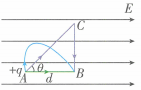
\includegraphics[width=0.3\linewidth]{Pic1.png}
\end{figure}

特点：\textbf{电场力做功与路径无关，只与初、末位置有关}。

\smallskip

公式：

\textcircled{1}.$W=qEd$，其中$d$为电荷沿电场方向的移动距离，注意不是两点距离！

\textcircled{2}.$W=qU$，其中$U$为两点间的电势差。

\subsubsection{电场力做功和电势能的关系}

1.\textbf{$W_{AB}>0\Longrightarrow E_{pA}>E_{pB}$}，\textbf{电场力做正功，电势能减小}。

2.\textbf{$W_{AB}<0\Longrightarrow E_{pA}<E_{pB}$}，电场力做负功，电势能增大。

3.电势能是\textbf{相对}的，与选取的\textbf{零势能面}有关。

4.电势能为电荷和对它作用的电场组成的系统所共有的。

5.电势能是标量。

\subsubsection{电势能的大小}

\begin{figure}[h]
\centering
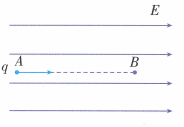
\includegraphics[width=0.3\linewidth]{Pic2.png}
\end{figure}

从$A\Longrightarrow B$电场力所做的功为$W_{AB}=E_{pA}-E_{pB}$。

若$A$点在零势能面上，$E_{pA}=0$，则$E_{pB}=-W_{AB}$。

\subsection{电势与等势面}

\subsubsection{电势}

电势：试探电荷在电场中某点具有的电势能$E_{p}$与它的电荷量$q$的比值，用$\psi$表示，单位是伏特。

\smallskip

公式(注意电势有负有正，需要代入物理量的正负)：

\begin{equation*}
    \centering
    \psi=\frac{E_{p}}{q}
\end{equation*}

标矢性：电势是标量。

相对性：同一点的电势随着零势能面的选取不同而不同，无提及情况下\textbf{默认无限远处/大地表面为零势能点(面)}。

\bigskip

\textbf{沿着电场线的方向，电势逐渐降低}。

\subsubsection{电势能与电势的关系}

1.\textbf{正电荷}$q>0$，则$\psi\geq0$时$E_{p}\geq0$，\textbf{电势越高，电势能越大}。

2.负电荷$q>0$，则$\psi\leq0$时$E_{p}\leq0$，电势越高，电势能越小。

\subsubsection{等势面}

等势面：电场中电势相等的各点组成的面。

特点：

1.\textbf{等势面一定与电场线垂直，即跟场强的方向垂直}。

2.\textbf{电荷在等势面上移动时不做功}。

3.\textbf{电场线总是从电势高的等势面指向电势低的等势面}。

4.\textbf{等差等势面越密集的地方，电场强度越大}。

\newpage

\subsection{特殊电场的等势面}

\subsubsection{点电荷的等势面}

\begin{figure}[h]
\centering
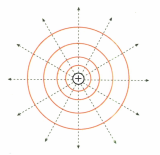
\includegraphics[width=0.3\linewidth]{Pic3.png}
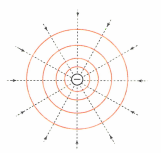
\includegraphics[width=0.3\linewidth]{Pic4.png}
\caption{正、负电荷电场的等势面}
\end{figure}

1.实质：是以点电荷为球心的一组同心球面。

2.等差等势面随着球面的半径增大而变得稀疏。

3.正点电荷的电场中，\textbf{距离场源电荷越近，电势越高}。取无限远处电势为零时，正场源电荷电场中的各点电势均大于零。

\subsubsection{匀强电场的等势面}

\begin{figure}[h]
\centering
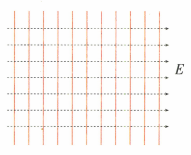
\includegraphics[width=0.3\linewidth]{Pic5.png}
\caption{匀强电场的等势面}
\end{figure}

1.实质：一簇垂直于电场线的平面。

2.等差等势面是互相平行、间距相等的平面。

\newpage

\subsubsection{等量同种点电荷的等势面}

\begin{figure}[h]
\centering
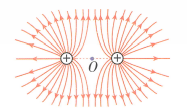
\includegraphics[width=0.3\linewidth]{Pic6.png}
\caption{等量同种正点电荷的电场线}
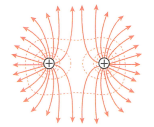
\includegraphics[width=0.3\linewidth]{Pic7.png}
\caption{等量同种正点电荷的等势面}
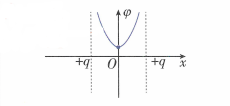
\includegraphics[width=0.4\linewidth]{Pic8.png}
\caption{等量同种正点电荷的两点连线上的电势特点}
\end{figure}

中点$O$处电势最低，其他点左右对称，且高于$O$点对称。

\begin{figure}[h]
\centering
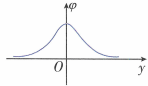
\includegraphics[width=0.3\linewidth]{Pic9.png}
\caption{等量同种正点电荷的连线的中垂线上的电势特点}
\end{figure}

中点$O$处电势最高，由中点到无限远处，电势一直降低，左右对称。

\newpage

\subsubsection{等量异种点电荷的等势面}

\begin{figure}[h]
\centering
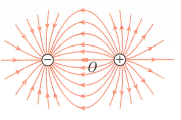
\includegraphics[width=0.3\linewidth]{Pic10.png}
\caption{等量异种正点电荷的电场线}
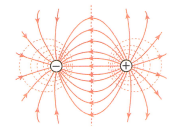
\includegraphics[width=0.3\linewidth]{Pic11.png}
\caption{等量异种正点电荷的等势面}
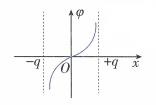
\includegraphics[width=0.3\linewidth]{Pic12.png}
\caption{等量异种正点电荷的两点连线上的电势特点}
\end{figure}

中点$O$处电势为零，由负点电荷到正点电荷处电势逐渐升高。

等量异种点电荷的连线的中垂线上的电势均为零。

\subsubsection{任意形状带电体的电场的等势面}

\begin{figure}[h]
\centering
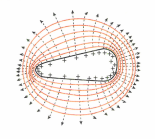
\includegraphics[width=0.3\linewidth]{Pic13.png}
\caption{任意形状带电体形成的电场的等势面}
\end{figure}

1.越接近带电体，等势面的形状越接近带电体外表面形状；越远离带电体，等势面形状越接近于球面。

2.\textbf{导体表面越尖锐的位置，电场线越密集}。

3.导体表面附近，\textbf{电场线与导体表面互相垂直}。

\subsection{概念辨析}

关于电场强度、电势、电势差、电势能的比较：

\begin{table}[h]
    \centering
    \begin{tabular}{c|c|c|c|c}
        \hline
         & 电场强度 & 电势 & 电势差 & 电势能 \\
        \hline
         & & & &\\
        定义式 & $E=\frac{F}{q}$ & $\psi=\frac{E_{p}}{q}$ & $U_{AB}=\frac{W_{AB}}{q}$ & $E_{p}=\psi q$\\
         & & & &\\
        \hline
        \makecell{决定\\因素} & \makecell{由电场本身决定\\与试探电荷无关} & \makecell{由电场本身决定\\与试探电荷无关\\大小具有相对性} & \makecell{由电场内两点间差异决定\\与试探电荷无关\\与参考点选择无关} & \makecell{由点电荷量和电势决定\\与参考点选取有关\\有相对性}\\
        \hline
        关系 & \makecell{电场为零\\电势不一定为零} & \makecell{电势为零\\电场不一定为零} & \makecell{电场为零的区域\\两点电势差一定为零\\\,\\电势差为零的两点间\\电场强度不一定为零} & \makecell{电场为零\\电势能不一定为零\\\,\\电势为零\\电势能一定为零}\\
        \hline
    \end{tabular}
\end{table}

\subsection{计算电场力做功的方法}

1.根据功的定义式$W=qEx$，其中$x$为初末位置沿电场线的位移差。

2.根据$W_{AB}=qU_{AB}$计算，注意判断做功和电势的正负性。

3.根据电场力做功与电势能的变化计算。

\begin{equation*}
    \centering
    W_{AB}=E_{pA}-E_{pB}=-(E_{pB}-E_{pA})=q\psi_{A}-q\psi_{B}
\end{equation*}

4.根据动能定理计算：$W+W_{0}=\Delta E_{k}$，其中$W$是电场力总共，$W_0$是其他力做功。

\subsection{电场的图像}

\subsubsection{$v-t$图像}

1.利用速度的变化确定动能的变化、合力的做功情况。

2.利用图像上某点\textbf{切线斜率}$\frac{\Delta v}{\Delta t}=a$，可以确定\textbf{加速度大小、合力大小、合力方向变化}，从而确定\textbf{电场方向、电势高低、电势能的变化}。

\subsubsection{$v-x$图像}

1.利用速度变化可确定动能变化、合力做功的情况。

2.利用图像上某点\textbf{切线斜率}$\frac{\Delta v}{\Delta x}=\frac{a}{v}$，可以确定\textbf{加速度情况、合力大小、合理方向变化}，从而确定\textbf{电场方向、电势高低、电势能的变化}。

\subsubsection{$\psi-x$图像}

1.利用纵坐标直接确定电势高低，结合电荷正负性确定电势能高低，再结合功能关系确定电场力的做功。

2.利用图像上某点\textbf{切线斜率}可确定\textbf{场强}，\textbf{斜率的绝对值决定场强大小}，\textbf{斜率的正负决定场强方向}，图像\textbf{极值点处场强为零}。

\subsubsection{$E-x$图像}

1.利用纵坐标直接确定场强大小和方向，从而判断电势变化，再结合粒子正负和大小确定\textbf{电场力的大小和方向}。

2.利用图像和横轴间的面积可以判断\textbf{电势差的大小}。

\subsubsection{$E_{p}-x$图像}

1.利用纵坐标可以直接确定电势能及其变化情况，从而判断电场力做功情况，结合粒子电荷量\textbf{确定电势的情况}。

2.利用图像上某点的\textbf{切线斜率}$\frac{\Delta E_{p}}{\Delta x}=qE$可以确定\textbf{电场力大小(或沿$x$轴方向的电场力分量大小)}，结合粒子电荷量可以确定\textbf{电场强度的分布情况}；再结合受力确定\textbf{加速度变化情况}，结合能量守恒/动能定理确定\textbf{动能变化情况}。


\newpage

\subsection{课后习题}

\begin{figure}[h]
\centering
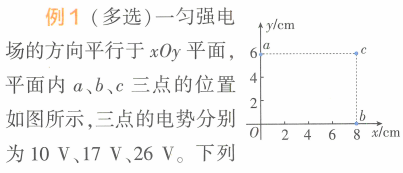
\includegraphics[width=0.6\linewidth]{Q1-1.png}
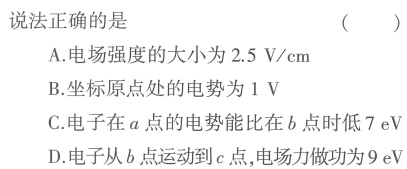
\includegraphics[width=0.6\linewidth]{Q1-2.png}
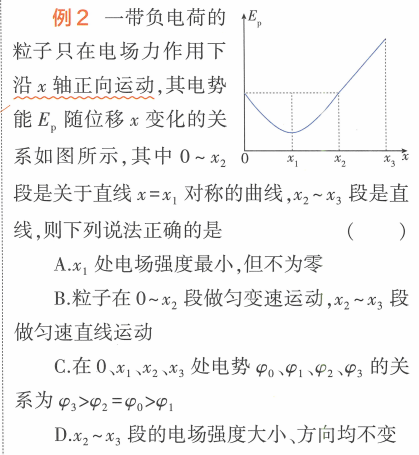
\includegraphics[width=0.6\linewidth]{Q2.png}
\end{figure}

\newpage

\begin{figure}[h]
\centering
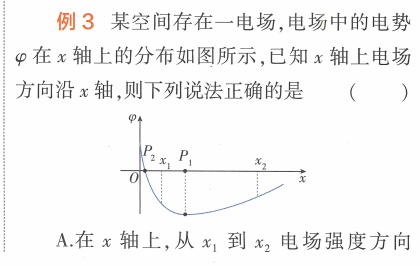
\includegraphics[width=0.6\linewidth]{Q3-1.png}
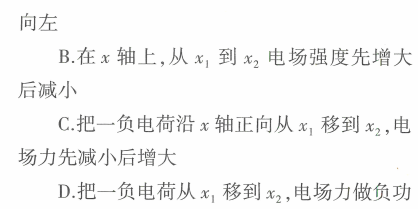
\includegraphics[width=0.6\linewidth]{Q3-2.png}
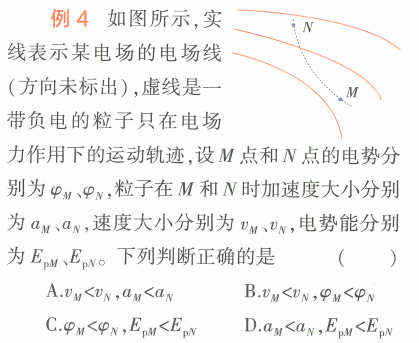
\includegraphics[width=0.6\linewidth]{Q4.png}
\end{figure}

\end{document}